%%%%%%%%%%%%%%%%%%%%%%%%%%%%%%%%%%%%%%%%%
% "ModernCV" CV and Cover Letter
% LaTeX Template
% Version 1.1 (9/12/12)
%
% This template has been downloaded from:
% http://www.LaTeXTemplates.com
%
% Original author:
% Xavier Danaux (xdanaux@gmail.com)
%
% License:
% CC BY-NC-SA 3.0 (http://creativecommons.org/licenses/by-nc-sa/3.0/)
%
% Important note:
% This template requires the moderncv.cls and .sty files to be in the same 
% directory as this .tex file. These files provide the resume style and themes 
% used for structuring the document.
%
%%%%%%%%%%%%%%%%%%%%%%%%%%%%%%%%%%%%%%%%%

%----------------------------------------------------------------------------------------
%	PACKAGES AND OTHER DOCUMENT CONFIGURATIONS
%----------------------------------------------------------------------------------------

\documentclass[11pt,a4paper,sans]{moderncv} % Font sizes: 10, 11, or 12; paper sizes: a4paper, letterpaper, a5paper, legalpaper, executivepaper or landscape; font families: sans or roman

\moderncvstyle{classic} % CV theme - options include: 'casual' (default), 'classic', 'oldstyle' and 'banking'
\moderncvcolor{purple} % CV color - options include: 'blue' (default), 'orange', 'green', 'red', 'purple', 'grey' and 'black'
%\usepackage[italian]{babel}
\usepackage[utf8]{inputenc}
\usepackage{lmodern}
\usepackage{enumitem}
\usepackage{fontawesome5}
\usepackage{ragged2e}

\usepackage[scale=0.9, top=1cm, bottom=3cm]{geometry} % Reduce document margins
\setlength{\hintscolumnwidth}{4cm} % Uncomment to change the width of the dates column
%\setlength{\makecvtitlenamewidth}{10cm} % For the 'classic' style, uncomment to adjust the width of the space allocated to your name

%----------------------------------------------------------------------------------------
%	NAME AND CONTACT INFORMATION SECTION
%----------------------------------------------------------------------------------------

\firstname{Francesco} % Your first name
\familyname{Dondi} % Your last name

% All information in this block is optional, comment out any lines you don't need
\title{Curriculum Vit\ae{}}
\mobile{+41 76456 50 32\hfill\ }
\email{francesco314@gmail.com\hfill\ }
\social[linkedin]{francesco-dondi\hfill\ } 
\address{8810 Horgen, ZH \hfill\ }
\extrainfo{\faIcon{birthday-cake} Born 1990, Italy, Italian citizen\hfill\  \\ \faIcon{plus-square} Swiss C permit until 30.09.27 \hfill\ \\ \faIcon{globe} German B1\hfill\ }
\photo[100pt][0pt]{me.jpg} % The first bracket is the picture height, the second is the thickness of the frame around the picture (0pt for no frame)
%\quote{"A Florence on raconte \\ que la Terre serait ronde"}

%----------------------------------------------------------------------------------------

\begin{document}

\makecvtitle % Print the CV title

\section{Professional Experience}

\cventry{06/2021 - 09/2022 \\ \textbf{Firebolt} \\ Fully Remote}{Software Developer}{}{}{}{Maintinaing and developing the SQL optimization engine and testing infrastructure.
\begin{itemize}
\setlength\itemsep{-0.3em}
\item Expanded supported SQL syntax and optimizations
\item reworked the test framework to support new test suite
\item contributed to rewriting to higher standards the optimization engine 
\end{itemize}
}
\cventry{08/2020 - 02/2021 \\ \textbf{F-Trust} \\ Zug / 50\% Remote}{Developer / Analyst}{}{}{}{
\begin{itemize}
\setlength\itemsep{-0.3em}
\item Maintained and developed a Trading Engine (C++)
\item redesigned, implemented and migrated product storage (PostgreSQL)
\item extracted and integrated data from multiple log streams
\item analyzed said data to highlight opportunities for improvement (Julia)
\end{itemize}
}
\cventry{10/2017 - 05/2020 \\ \textbf{Google} \\ Zürich / 10\% Remote}{Software Developer}{}{}{}{Within Search, productionized an initially experimental tool (C++).
\begin{itemize}
\setlength\itemsep{-0.3em}
\item Improved runtime from days to hours
\item added support for new kinds of data
\item made the results easily visualizable and monitorable
\item made onboarding orders of magnitude faster for most cases
\end{itemize}
}
\cventry{04/2016 - 10/2017 \\ \textbf{Ascent Software} \\ Luqa(Malta)}{Software Developer}{}{}{}{Bridging from internal API to new device API for automotive.}
\cventry{04/2015 - 04/2016 \\ \textbf{Rulex Inc.}/\textbf{CNR} \\ Genova (Italy)}{Junior Developer}{}{Genua (Italy)}{}{Reworked C/MATLAB algorithms for OpenMP/CUDA parallelization}

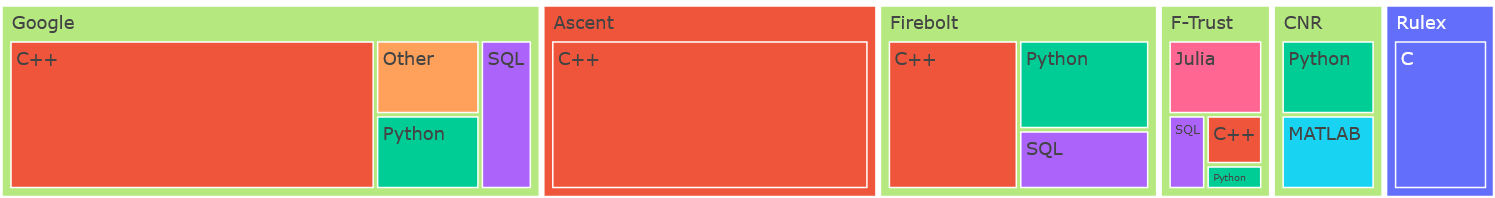
\includegraphics[scale=0.5]{languages.png}

\section{Education}

\cventry{2009--2015}{\href{http://www.unipd-scuolagalileiana.it/en/}{Galileian School of Higher Education}}{University of Padua}{Enriching program for gifted students}{\textit{98/100}}{}
\cventry{2012--2014}{Master Degree in Mathematics}{University of Padua}{}{\textit{108/110}}{}
\cventry{2009--2012}{Bachelor Degree in Mathematics}{University of Padua}{}{\textit{110/110 cum Laude}}{}
\cventry{2004--2009}{High School - Science Track, with added French and IT}{Liceo E. Fermi}{Bologna}{\textit{100/100 cum Laude}}{}

\section{Skills}

\subsection{Programming languages} 
\cvitem{Primary}{\begin{description}[nosep,after=\leavevmode\vspace*{-1\baselineskip},labelwidth = 100pt] 
					\item[High Performance] \textsc{C/C++} {\small(up to \textsc{C++20})}
					\item[Advanced Scripting] \textsc{Julia}
					\item[Database] \textsc{SQL (PostgreSQL)}
			    \end{description}}
\cvitem{Confident}{\textsc{Java}, \textsc{C}, \textsc{Javascript}, \textsc{BASH}, \textsc{Python}, \textsc{MATLAB}}
\cvitem{Interested in}{\textsc{Rust}, \textsc{F$\sharp$}, \textsc{Go}, \textsc{Scala}, \textsc{Haskell}}
\cvitem{Frameworks}{\href{https://www.polymer-project.org/}{\textsc{Polymer}}, \href{https://github.com/abseil/abseil-cpp}{\textsc{Abseil}}, \href{https://www.boost.org/}{\textsc{Boost}}, \href{https://developer.nvidia.com/cuda-zone}{\textsc{Nvidia CUDA}}, \href{https://www.openmp.org/}{\textsc{OpenMP}}}


\subsection{Tools}
\cvitem{Organization}{\href{https://weekdone.com/resources/objectives-key-results}{OKRs}, Agile, Test Driven Development}
\cvitem{Writing}{Technical and collaborative documents}
\cvitem{Editors}{\textsc{Vim}, Visual Studio, Eclipse, TexMaker for \LaTeX, [Google internal]}
\cvitem{Versioning}{Git, SVN, [Google internal] }
\cvitem{Debug}{GDB, Valgrind, [Google internal]}
\cvitem{Profiling}{Valgrind, \href{http://www.brendangregg.com/flamegraphs.html}{Flamegraph}}
\cvitem{Orchestration}{\href{https://en.wikipedia.org/wiki/Kubernetes}{Borg (model of Kubernetes)}}
\cvitem{Data presentation}{\href{https://marketingplatform.google.com/about/data-studio/}{Google Data Studio}, \textsc{Julia} Plot modules}

\section{Language}

\cventry{2022-2023}{In-person intensive course, level A2-B1}{German}{Zürich}{}{}
\cventry{2018}{In-person private course level A2}{German}{Zürich}{}{}
\cventry{2009}{English course with Home-stay}{English}{York}{}{}
\cventry{2005}{Cultural exchange}{French}{Marseille}{}{}

\subsection{Levels}

\cvitemwithcomment{Italian}{Mother tongue}{}
\cvitemwithcomment{English}{Advanced}{110/120 TOEFL}
\cvitemwithcomment{French}{Intermediate}{Good understanding, understandable conversation}
\cvitemwithcomment{German}{Good}{B1 level}

\section{More}
{\small

\subsection{Awards}

\cvitem{2014}{ GRE test score: Verbal 165 ($95^\circ$ percentile), Quantitative : 170 ($98^\circ$ percentile), Analytical: 4.0 ($56^\circ$ percentile }
\cvitem{2009}{Italian Olympics of Mathematics: Gold}
\cvitem{2008}{Italian Olympics of Information Technology: Bronze}
\cvitem{2006}{Special mention in high school literary prize ``Le ali dell'Ippogrifo''}

\subsection{Hackatons}

\cvitem{12-13/12/15}{\href{https://www.h-farm.com/en}{H-Farm} H-Ack Luxottica: ideas for the future of glasses. } 
\cvitem{19-20/03/16}{\href{https://www.h-farm.com/en}{H-Farm} H-Ack Food: reinventing the 'Bio food' experience. }
}
\end{document}
